\chapter{ミラー計測実験}
\thispagestyle{empty}
\label{chap5}
\graphicspath{{chap5/figure/}}
\minitoc

\newpage
%%%%%%%%%%%%%%%%%%%%%%%%%%%%%%%%%%%%%%%%%%%%%%%%%%%%%%%%%%%%%%%%%%%%%%%%%%%%%


% ================================================== %
% section
% ================================================== %
\section{諸言}
\label{chap5_introduction}

本章では、実際に天文用Wolterミラーを\ref{chap3}章の提案手法による計測実験を行い、その解析を行う。
測定対象となるミラーは、東京大学の三村グループによって作製された3枚の天文用Wolterミラー(表\ref{tb:fabricated_wolter_mirror_list})であり、これらの設計パラメータは1章\ref{chap1_wolter_arrangement}に示した通りである。
この3枚のミラーそれぞれについて位相回復計算を行った結果およびそこから計算される形状誤差について述べる。
続いて、これらは既に真円度測定がなされているため、本実験での計測結果と真円度測定結果との比較・検討を行う。
また、2021年1月のミラーについて繰り返し計測および光軸周りの設置角度を変えた置き直し計測を行い、その精度についても検討する。

\begin{table}[h]
\begin{center}
  \begin{tabular}{|c|c|} \hline
    番号 & 作製年月 \\ \hline
    1 & 2020年 2月 \\
    2 & 2020年 9月 \\
    3 & 2021年 1月 \\ \hline
  \end{tabular}
  \caption{三村グループにより作製されたWolterミラー}
  \label{tb:fabricated_wolter_mirror_list}
\end{center}
\end{table}

\clearpage
% ================================================== %
% section
% ================================================== %
\newpage

\section{実験の構成}

実験装置の概要を図\ref{fig:mirror_experiment_schematic}に示す。
まず、レーザーからビームを出力し、これをNDフィルタによって減衰させ、強度を調整する。
次に、レンズを2つ使ってビームを拡大し平行化する。
これを測定対象のWolterミラーに入射し、さらにタイコグラフィのための回転ピンホールを通過させる。
最後に、一番下流にあるCCDカメラで強度分布を撮影する。

\begin{figure}[!ht]
\centering
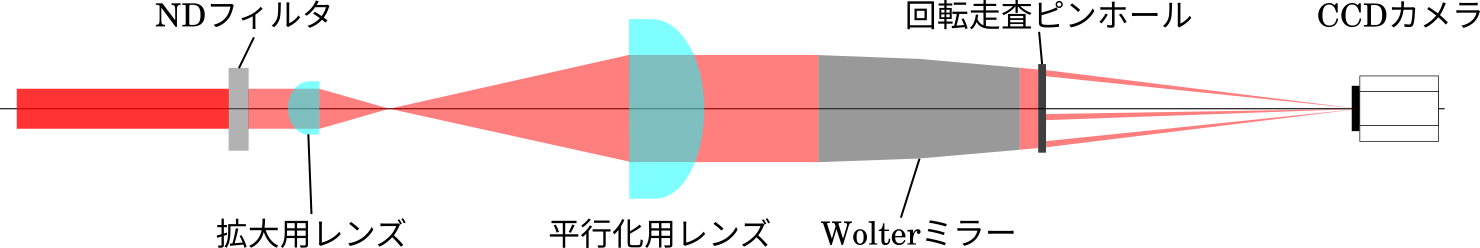
\includegraphics[width=13cm]{mirror_experiment_schematic.png}
\caption{ミラー測定実験系 模式図}
\label{fig:mirror_experiment_schematic}
\end{figure}

これらの光学素子のパラメータを表\ref{tb:mirror_experiment_params}に示す。
なお、NDフィルタは実験によって適宜ピークがダイナミックレンジに収まるように設定されるため、そのパラメータ等を記述しない。

\begin{table}[h]
\begin{center}
  \begin{tabular}{|c|c|} \hline
    パラメータ & 値 \\ \hline
    ビーム波長 & 632.8 nm  \\
    ビームサイズ($\text{TEM}_{00} 1/e^2$点 +3\%) & 0.63 mm  \\
    ビーム発散角度($\text{TEM}_{00}$ +3\%) & 1.3 mrad  \\
    拡大用レンズ焦点距離 & 8.0 mm  \\
    平行化用レンズ焦点距離 & 800.0 mm  \\
    拡大倍率 & 100 倍 \\
    レンズ設計波長 & 541.6 nm \\ \hline
  \end{tabular}
  \caption{Wolterミラー計測実験装置における各素子のパラメータ}
  \label{tb:mirror_experiment_params}
\end{center}
\end{table}

これらを構成した実験装置のCAD図を以下に示す。図\ref{fig:mirror_experiment_asm_cad_side}が横から見た図、図\ref{fig:mirror_experiment_asm_cad_isometric}が俯瞰して見た図である。

\begin{figure}[!ht]
\centering
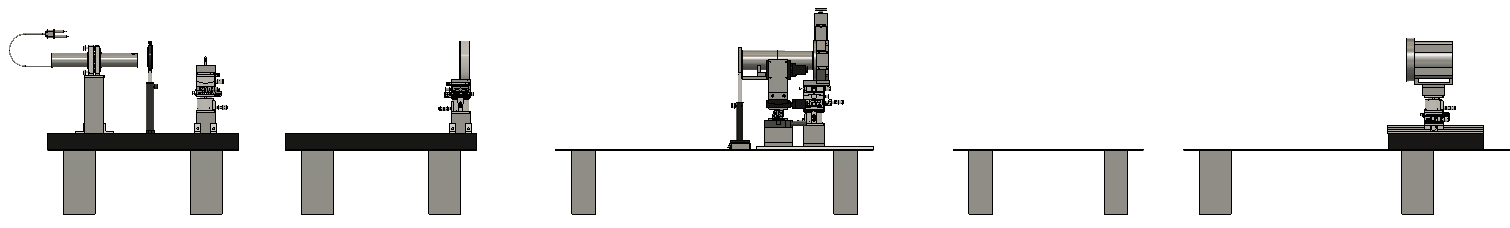
\includegraphics[width=14cm]{asm_total_side.png}
\caption{ミラー測定実験系 側面図}
\label{fig:mirror_experiment_asm_cad_side}
\end{figure}

\begin{figure}[!ht]
\centering
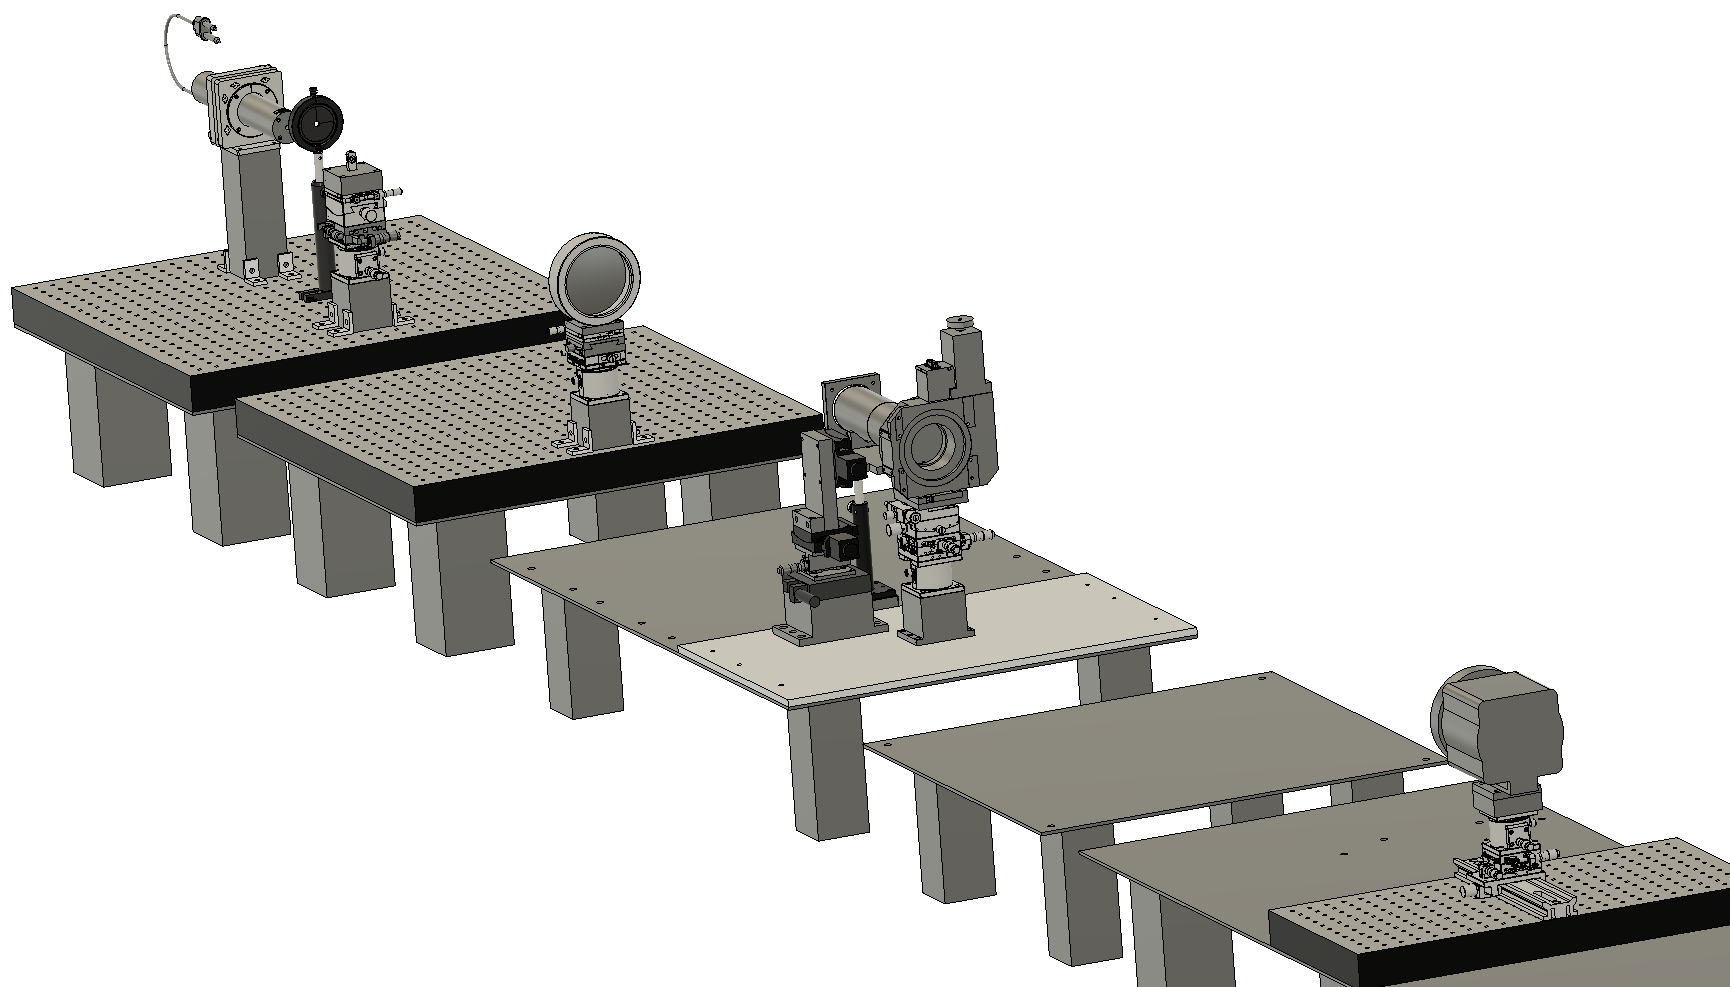
\includegraphics[width=10cm]{asm_total_isometric.png}
\caption{ミラー測定実験系 俯瞰図}
\label{fig:mirror_experiment_asm_cad_isometric}
\end{figure}

\subsection{ミラーの把持}
回転体ミラーの測定実験系を構成する上で、ミラーの把持は一つの問題となる。
板型ミラーの場合であれば、反射面以外の平面部を挟むようにして把持することができる。
一方で円筒型の薄いミラーの場合そのような部分はなく、できるだけ小さな応力で、かつ設置位置に決まった位置に収まるように把持しなければならない。
そこで、仙波らの方法にならい、Bessel点で触れるように下から把持する機構を採用する。\cite{Senba2010}
Bessel点は均等荷重を受ける2点支持された梁の重力によるたわみ量が最小となるような点であり、梁の全長$L$に対して、梁の両端から内側に向かって約$0.2203L$(あるいは中心から$\pm 0.2797 L$)の位置として計算される。
ミラーは光軸上の位置によって半径が異なり厳密には均等荷重ではないが、斜入射が小さくほぼ真円筒とみなせるため、近似的な範囲ではこれで十分であると考えた。
測定対象のミラー全長220 mmに対してBessel点は中心から約$\pm$61.53 mmであり、これを採用した把持機構は図\ref{fig:mirror_holder_jig}のようになった。
ミラーと治具の接触点は赤点で示す通りである。

\begin{figure}[!ht]
\centering
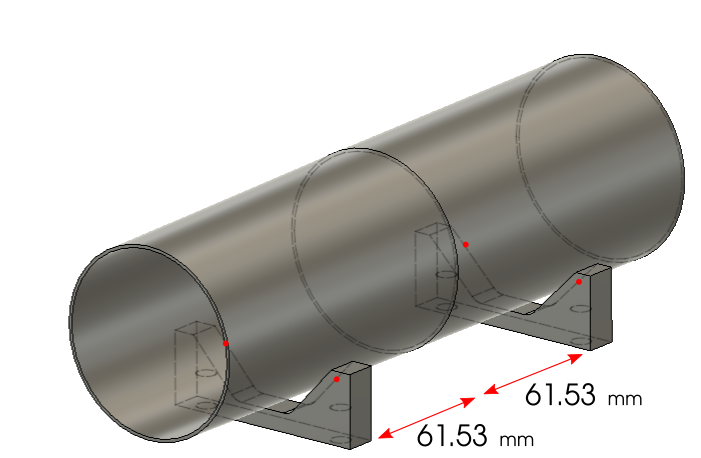
\includegraphics[width=10cm]{mirror_holder_jig.png}
\caption{ミラー把持部の設計図}
\label{fig:mirror_holder_jig}
\end{figure}

\subsection{ピンホールの設計}

ピンホールの設計は図\ref{fig:mirror_pinhole_arrangement}に示す通りである。
断りとして、以下の設計が2つの誤謬を孕んでいることを述べておく。
1つは、ピンホール中心が移動する円の直径はちょうど計測する輪帯状波面のちょうど半分の直径とするのが自然だが、そのような直径を持つ円に対して1つのピンホールが対応する角度を先に決めて、その角度を持つ扇形の弦が直径となるように円を定めている。
もう1つは、シミュレーション上で回復ができると判断した半径2.25 mmの円に対して、直径2.25 mmとしてしまったことである。
これによって、上の計算にはもはや意味を失っている。
ただ、測定対象の輪帯がピンホール通過領域に収まれば問題はなく、直径の決め方は些細な問題である。

\begin{figure}[!ht]
\centering

\subfloat[ピンホールの設計]{
    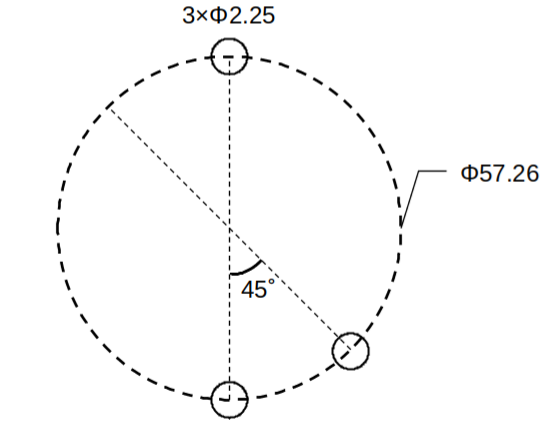
\includegraphics[width=7cm]{pinhole_arrangement.png}
    \label{fig:mirror_pinhole_arrangement}
}
\subfloat[回転半径の決め方]{
    \centering
    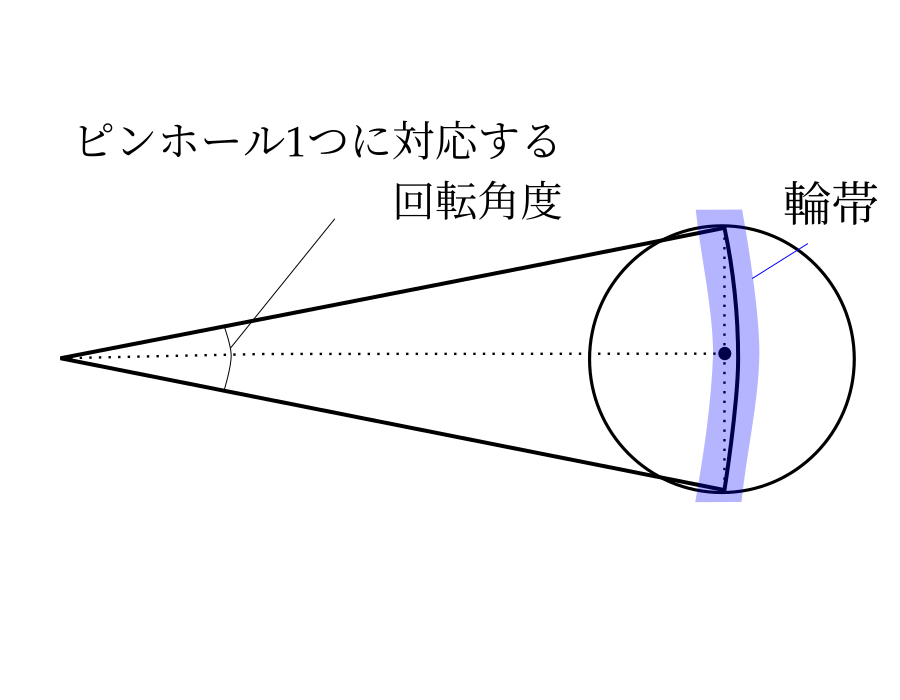
\includegraphics[width=6cm]{pinhole_arrangement_policy.png}
    \label{fig:mirror_pinhole_arrangement_policy}
}
\caption[]{ピンホールの設計}
\label{fig:pinhole_arrangement_pictures}
\end{figure}


\clearpage
% ================================================== %
% section
% ================================================== %
\newpage

\section{計測波面以外の通過光の処理方法に関する検討}
測定対象となっている天文用Wolterミラーは、X線集光用に設計・作製されたものであり、可視光を入射した際にどのような集光波面が生じるかは未検討である。
特に、可視光はX線に比べ2桁程度波長が長く、回折の影響が顕著であることが大きな差異として存在する。
\ref{chap4}章での提案手法の検討は、あくまで波面計測の対象である輪帯のみが存在する場合について行われたが、実際にミラーを計測する実験においては測定対象以外の光も通過してCCDカメラの方向に進行する。
円盤状に広がる平行光を入射した際にミラーより下流に通過する光は、図\ref{fig:mirror_beam_path_types}に示す通り4種類存在する。

図\ref{fig:mirror_beam_path_types}(a)が、測定対象となる波面、つまり正しく放物面、双曲面の順に2回反射した光である。
これに対して、図\ref{fig:mirror_beam_path_types}(b)の直接通過してCCDカメラに到達する光、
図\ref{fig:mirror_beam_path_types}(c)の放物面に当たらず直接双曲面で反射された光、
図\ref{fig:mirror_beam_path_types}(d)の開口端のエッジで回折して進行する光が存在する。

\begin{figure}[!ht]
\centering
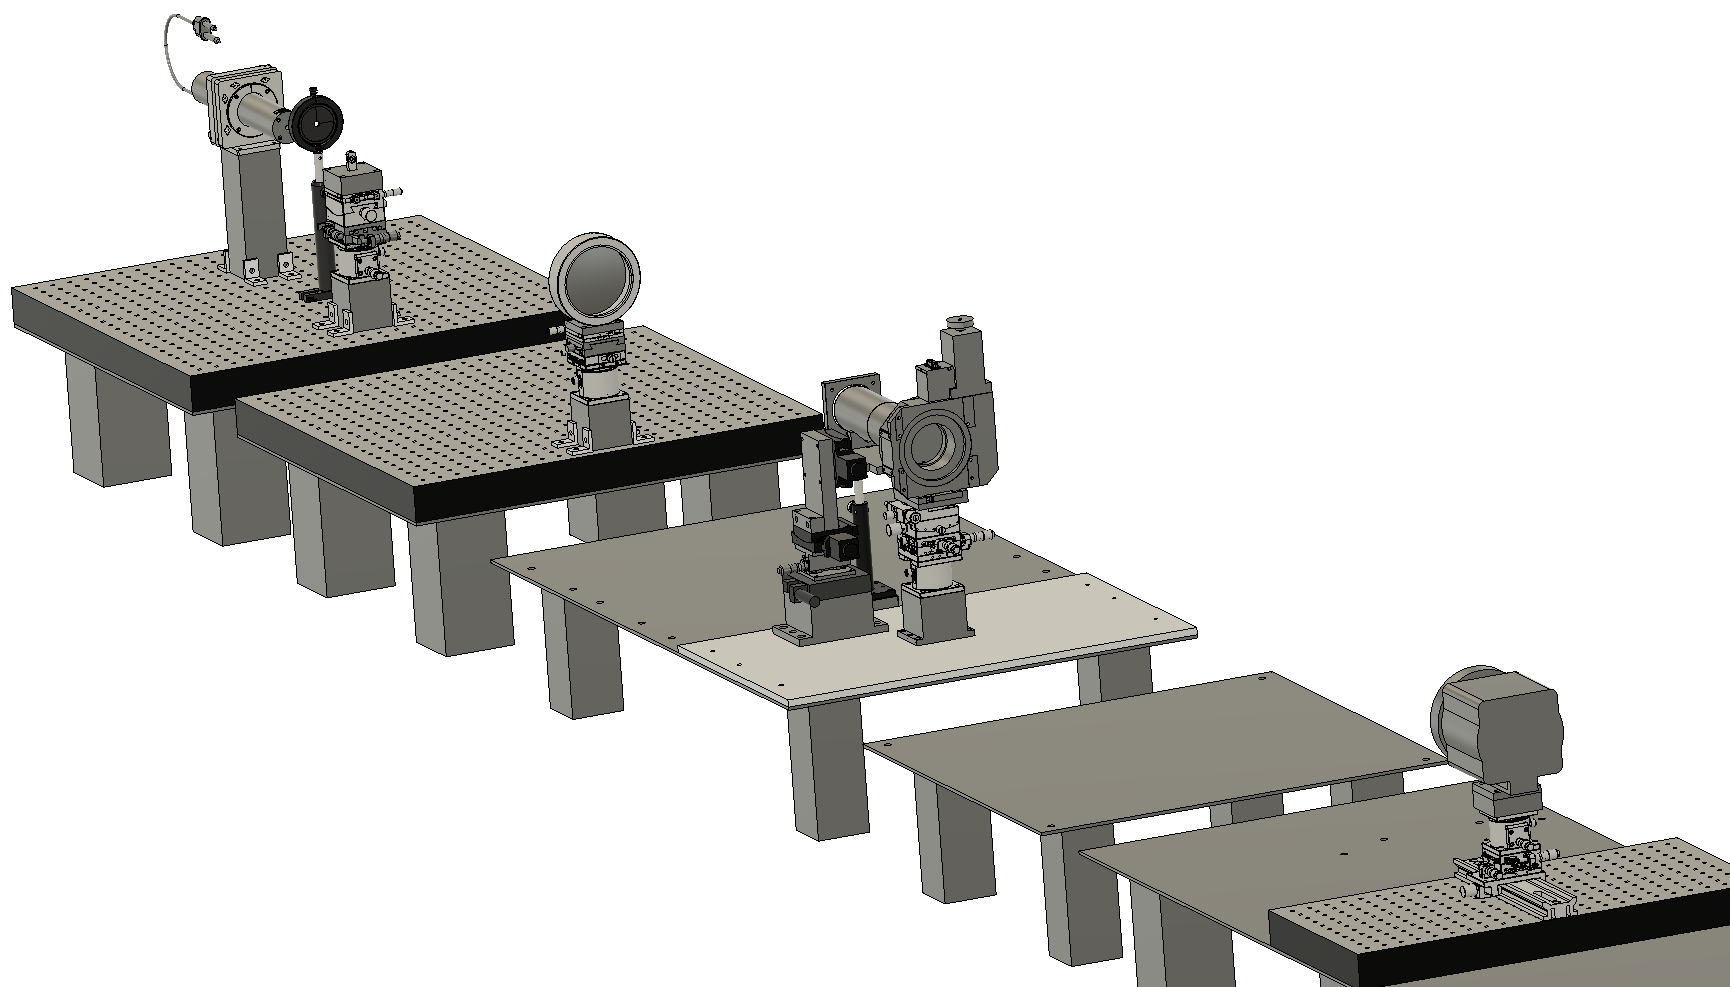
\includegraphics[width=10cm]{asm_total_isometric.png}
\caption{ミラーに入射した光の進路}
\label{fig:mirror_beam_path_types}
\end{figure}

直接通過光は、
\subsection{直接通過光}


\subsection{双曲面で1回反射した光}


\subsection{上流端エッジでの回折光}
\label{chap5_}

\clearpage
% ================================================== %
% section
% ================================================== %
\newpage

\section{撮影条件および撮影像の前処理}

撮影時の条件を表

\begin{table}[!ht]
\begin{center}
  \begin{tabular}{|c|c|} \hline
    パラメータ & 値 \\ \hline
    温度 & \SI{20}{\degreeCelsius}  \\
    CCDカメラ設定温度 & \SI{15}{\degreeCelsius} \\
    設計波長 & 541.6 nm \\ \hline
  \end{tabular}
  \caption{Wolterミラー計測実験装置における各素子のパラメータ}
  \label{tb:mirror_experiment_params}
\end{center}
\end{table}


\clearpage
% ================================================== %
% section
% ================================================== %
\newpage

\section{可視光ビームによるWolterミラー集光波面強度分布の測定}



\clearpage

% ================================================== %
% section
% ================================================== %
\newpage

\section{下流端走査タイコグラフィの結果}

\clearpage
% ================================================== %
% section
% ================================================== %
\newpage

\section{回復波面の解析}
\subsection{周方向誤差の真円度測定結果との比較}

% ================================================== %
% section
% ================================================== %
\section{結論}
\label{chap5_conclusion}


%%%%%%%%%%%%%%%%%%%%%%%%%%%%%%%%%%%%%%%%%%%%%%%%%%%%%%%%%%%%%%%%%%%%%%%%%%%%%

%%% Local Variables:
%%% mode: katex
%%% TeX-master: "../thesis"
%%% End:
